\section{Proposta} % (fold)
\label{sub:proposta}
	
	O objetivo geral desse projeto é proporcionar ao usuário/cliente a oportunidade de limpar sua casa de forma cômoda e confortável para o mesmo. Este objetivo será alcançado através da remoção da poeira e/ou partículas de sujeira encontradas no cômodo da casa. A solução proposta neste projeto será a criação de um robô aspirador autônomo, que auxiliará na tarefa supracitada. 

	Tal robô terá capacidade de desviar os obstáculos encontrados durante seu percurso, além de ter autonomia de voltar à sua base quando necessário (ao término da tarefa ou quando sua bateria estiver prestes a acabar), a fim de se carregar.

	Esta solução está organizada segundo a EAP (Estrutura analítica do projeto) apresentada na Figura \ref{img:eap}, destacando os entregáveis e seus subsistemas ao longo de todo o projeto.
	
	\begin{figure}[H]
		\centering
		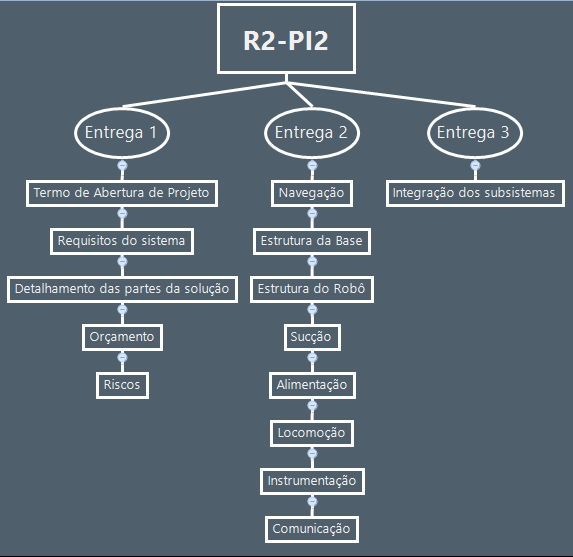
\includegraphics[scale=0.55]{figuras/eap.png}
		\caption{Estrutura Analítica do Projeto do R2-PI2.}
		\label{img:eap}
	\end{figure}

	A primeira entrega trata basicamente do gerenciamento do projeto. Tal etapa é de suma importância para o andamento do projeto, visto que nela será definida a solução para o problema exposto, assim como os requisitos necessários para atingir tal objetivo com total eficiência.

	Vale observar que, analisando a EAP, fica evidente como foi feita a separação dos subsistemas do produto final (a ser obtido na Entrega 3). O desmembramento facilita o trabalho ao longo do curso do projeto. Porém vale lembrar que os subsistemas, mesmo produzidos separadamente, devem  andar em total harmonia, a fim de alcançar o objetivo final.
% subsection proposta (end)
